\documentclass[12pt,spanish]{article}

\usepackage[left=2.5cm,right=2cm,top=2cm,bottom=2cm]{geometry}
\setlength{\parindent}{0mm}

\usepackage{float}

\usepackage{parskip}
\usepackage[document]{ragged2e}
\usepackage{babel}
\usepackage[utf8]{inputenc}
\usepackage{amsmath,amsthm,mathtools}
\usepackage{amsfonts,amssymb,latexsym}
\usepackage{enumerate}
\usepackage[dvips,usenames]{color}
\definecolor{RojoAnayelRey}{rgb}{1,.25,.25}
\usepackage{tikz}
\usepackage[bookmarks=true,
            bookmarksnumbered=false, % true means bookmarks in 
                                     % left window are numbered                         
            bookmarksopen=false,     % true means only level 1
                                     % are displayed.
            colorlinks=true,
            urlcolor=cyan,
            linkcolor=webred]{hyperref}
            
\usepackage{beton}
\usepackage[T1]{fontenc}

% Theorem environments

%% \theoremstyle{plain} %% This is the default
\newtheorem{theorem}{Teorema}[section]
\newtheorem{corollary}[theorem]{Corolario}
\newtheorem{lemma}[theorem]{Lema}
\newtheorem{proposition}[theorem]{Proposici\'on}
%\newtheorem{ax}{Axioma}

\theoremstyle{definition}
\newtheorem{definition}{Definici\'on}[section]
\newtheorem{algorithm}{\textrm{\bf Algoritmo}}[section]

\theoremstyle{remark}
\newtheorem{remark}{Observaci\'on}
\newtheorem{example}{Ejemplo}
\newtheorem{exercise}{Ejercicio}
%\newenvironment{solution}{\begin{proof}[Solution]}{\end{proof}}
\newenvironment{solution}{\begin{proof}[Solución]}{\end{proof}}
\newtheorem*{notation}{Notaci\'on}


\title{Relación 1}

\author{David Cabezas Berrido}

\date{}

\begin{document}
\maketitle

\setcounter{exercise}{2}
\begin{exercise} %3

  Debemos tener en cuenta que $\alpha'(X-\mu)$ es una variable
  aleatoria unidimensional.
  
  Si $k=0$, el resultado es obvio: $E[1]=1$, ya que $m=\frac{k}{2}=0$
  y $0!=a^0=1$ para cualquier número real $a$. Suponemos en adelante
  $k>0$.
  
  Si $\alpha=0$, obtenemos otra trivialidad: $E[0]=0$. De lo
  contrario, podemos ver $\alpha'$ como una matriz $1\times p$ de
  rango máximo y aplicar el resultado sobre transformaciones lineales
  de rango máximo (RESULTADO 4 de DNM para $\Sigma>0$) para concluir
  $Y\sim
  N(\alpha'\mu-\alpha'\mu,\alpha'\Sigma\alpha'')=N(0,\alpha'\Sigma\alpha)$.
  
  El resultado auxiliar nos proporciona entonces $E[Y^k]=0$ para $k$
  impar y \\ $E[Y^k]=(\alpha'\Sigma\alpha)^\frac{k}{2} (k-1)!!$,
  sustituyendo $m=\frac{k}{2}$ obtenemos
  $E[Y^k]=(\alpha'\Sigma\alpha)^m (2m-1)!!$ y sólo queda probar
  $(2m-1)!!=\frac{(2m)!}{2^m m!}$ para todo $m\in\mathbb{N}$,
  $m\geq 1$. Esto lo haremos por inducción sobre $m$:
  
  En el caso $m=1$ basta desarrollar y obtenemos
  \[(2\cdot 1-1)!!=1!!=1;\qquad \frac{(2\cdot 1)!}{2^1
      1!}=\frac{2}{2}=1\] Supuesta la igualdad para $m-1$, es decir,
  \[(2m-3)!!=\big(2(m-1)-1\big)!!=\frac{\big(2(m-1)\big)!}{2^{m-1} (m-1)!}=\frac{(2m-2)!}{2^{m-1} (m-1)!}.\]

  Comprobamos para $m$,
  \begin{align*}
    &(2m-1)!!=\frac{(2m)!}{2^m m!}
      \Longleftrightarrow (2m-1)(2m-3)!!=\frac{(2m)!}{2^m m!} \\
    \xLeftrightarrow[m-1]{\text{Caso}}\quad &(2m-1)\frac{(2m-2)!}{2^{m-1}(m-1)!}=\frac{(2m)!}{2^m m!} \Longleftrightarrow (2m-1)!=\frac{(2m)!}{2m}
  \end{align*}
  y obtenemos lo que queríamos.
  
\end{exercise}

\setcounter{exercise}{4}
\begin{exercise} %5
  \[\Sigma=
    \begin{pmatrix}
      1 & 0 & \sigma_{13} \\
      0 & 1 & \sigma_{23} \\
      \sigma_{13} & \sigma_{23} & 1
    \end{pmatrix}
  \]

  Los menores de orden 1 y 2 de la diagonal principal de $\Sigma$
  valen los dos $1>0$, luego $\Sigma$ es definida positiva si, y solo
  si su determinante es positivo. Hemos de probar por tanto
  $0\geq|\Sigma|=1-\sigma_{13}^2-\sigma_{23}^2$, sabiendo que
  $\sigma_{13}+\sigma_{23}>\frac{3}{2}$. Por comodidad, renombramos
  $\sigma_{13}=x$, $\sigma_{23}=y$; queremos probar $x^2+y^2\geq 1$
  para $x+y>\frac{3}{2}$.

  Geométricamente, esto no es más que decir que el semiplano abierto
  $P:x+y>\frac{3}{2}$ está contenido en el complementario del disco
  abierto unidad $D:x^2+y^2 < 1$, o lo que es lo mismo,
  $P\cap D=\emptyset$. En esta figura se ve claramente
  \begin{figure}[H]
    \centering
    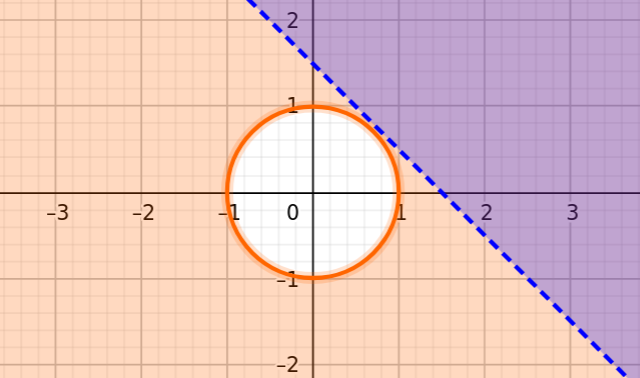
\includegraphics[width=80mm]{ej1-5.png}
  \end{figure}

  Haremos una demostración analítica, la función
  $f(x,y)=x^2+y^2\geq 0$ está minorada y por tanto tiene ínfimo no
  negativo en el conjunto $P$. Caben tres posibilidades:
  \begin{itemize}
  \item El ínfimo se alcanza en un punto interior donde se anula el
    gradiente, pero $\nabla f(x,y)=2(x,y)\neq(0,0)$ en $P$.
  \item El ínfimo se alcanza en la frontera de $P$, donde
    $y=\frac{3}{2}-x$. $f(x,\frac{3}{2}-x)=2x^2-3x+\frac{9}{4}$, que
    es mínimo en $x=\frac{3}{4}$ y vale $1.125>1$.
  \item Existe una sucesión divergente cuya imagen por $f$ converge al
    ínfimo, esto no puede darse puesto que $f$ es el cuadrado de la
    norma euclídea.
  \end{itemize}

  De esto deducimos que $\inf\{f(x,y) : (x,y)\in P\}=1.125$ y puesto
  que $P$ no contiene a su frontera, $x^2+y^2>1.125$ en todo $P$. Y
  por tanto $|\Sigma|\leq 0$, por lo que $\Sigma$ no puede ser
  definida positiva.
\end{exercise}

\setcounter{exercise}{6}
\begin{exercise}
  $Y\sim N_3(\mu,\Sigma)$, con
  \[\mu=
    \begin{pmatrix}
      3 \\
      1 \\
      4
    \end{pmatrix},\qquad \Sigma=
    \begin{pmatrix}
      6 & 1 & -2 \\
      1 & 13 & 4 \\
      -2 & 4 & 4
    \end{pmatrix}
  \]

  $|\Sigma|=144>0$ y $\Sigma$ simétrica. Luego es definida
  positiva. La idea de los apartados a-e es escribir la variable que
  queremos estudiar como una transformada lineal de rango máximo de
  $Y$ y aplicar el resultado de transformaciones lineales de rango
  máximo para $\Sigma>0$.
  
  \begin{enumerate}[a)]
  \item \[Z=2Y_1-Y_2+3Y_3=
      \begin{pmatrix}
        2 & -1 & 3
      \end{pmatrix}
      Y
    \]
    Como la matriz $B=\begin{pmatrix}
        2 & -1 & 3
      \end{pmatrix}$ tiene rango 1, el resultado sobre
      transformaciones lineales de máximo rango para $\Sigma>0$ nos
      asegura que $Z\sim N_1(B\mu,B\Sigma B')=N_1(17,21)$.
    \item $(Z_1,Z_2)$ donde $Z_1=Y_1+Y_2+Y_3$, $Z_2=Y_1-Y_2+2Y_3$.
      \[\begin{pmatrix}
          Z_1 \\
          Z_2
        \end{pmatrix}
        =\begin{pmatrix}
          1 & 1 & 1 \\
          1 & -1 & 2
        \end{pmatrix}Y=BY
      \]
      Esta vez el rango de $B=\begin{pmatrix}
          1 & 1 & 1 \\
          1 & -1 & 2
        \end{pmatrix}$ es 2, y el mismo resultado nos da \\ $\begin{pmatrix}
          Z_1 \\
          Z_2
        \end{pmatrix}\sim N_2\left(
        \begin{pmatrix}
          8 \\ 10
        \end{pmatrix},
        \begin{pmatrix}
          29 & -1 \\
          -1 & 9
        \end{pmatrix}\right)$.
      \item \[Y_2=
      \begin{pmatrix}
        0 & 1 & 0
      \end{pmatrix}
      Y=BY
    \]
    El rango de $B$ sigue siendo máximo, por tanto $Y_2\sim N_1(1,13)$.
    \item \[\begin{pmatrix}
          Y_1 \\
          Y_3
        \end{pmatrix}
        =\begin{pmatrix}
          1 & 0 & 0 \\
          0 & 0 & 1
        \end{pmatrix}Y\] Una vez más el mismo resultado nos dice
      que $\begin{pmatrix}
          Y_1 \\
          Y_2
        \end{pmatrix}\sim N_2\left(
        \begin{pmatrix}
          3 \\ 4
        \end{pmatrix},
        \begin{pmatrix}
          6 & -2 \\
          -2 & 4
        \end{pmatrix}\right)$.
      \item \[\begin{pmatrix}
          Y_1 \\
          Y_3 \\
          \frac{1}{2}(Y_1+Y_2)
        \end{pmatrix}
        =\begin{pmatrix}
          1 & 0 & 0 \\
          0 & 0 & 1 \\
          \frac{1}{2} & \frac{1}{2} & 0
        \end{pmatrix}Y\]
      $\begin{pmatrix}
         Y_1 \\
         Y_3 \\
         \frac{1}{2}(Y_1+Y_2)
        \end{pmatrix}\sim N_3\left(
        \begin{pmatrix}
          3 \\ 4 \\ 2
        \end{pmatrix},
        \begin{pmatrix}
          6 & -2 & \frac{7}{2} \\
          -2 & 4 & 1 \\
          \frac{7}{2} & 1 & \frac{21}{4}
        \end{pmatrix}\right)$.
    \item Encontrar $Z$ tal que $Z=(T')^{-1}(Y-\mu)\sim N_3(0,I)$. Con
      $T$ la matriz correspondiente a la factorización de Cholesky,
      $\Sigma=T'T$.

      Utilizamos el algoritmo para la descomposición de Cholesky
      implementado en la herramienta \href{https://www.sagemath.org}{\texttt{SageMath}}, y obtenemos
      que (redondeando)
      \[\Sigma=T'T=
        \begin{pmatrix}
          2.4495 & 0 & 0 \\
          0.4082 & 3.5824 & 0 \\
          -0.8165 & 1.2096 & 1.3675
        \end{pmatrix}
        \begin{pmatrix}
          2.4495 & 0.4082 & -0.8165 \\
          0 & 3.5824 & 1.2096 \\
          0 & 0 & 1.3675
        \end{pmatrix}
      \]
      También con \texttt{SageMath}, calculamos la inversa:
      \[T^{-1}=\begin{pmatrix}
          0.4082 & -0.0465 & 0.2849 \\
          0 & 0.2791 & -0.2469 \\
          0 & 0 & 0.7312
        \end{pmatrix}\]
      Luego \[Z=\begin{pmatrix}
          0.4082 & -0.0465 & 0.2849 \\
          0 & 0.2791 & -0.2469 \\
          0 & 0 & 0.7312
        \end{pmatrix}\left(Y-\mu\right)\]
      Como $T'T=\Sigma$, se tiene $Z\sim N_3(0,I)$.
    \item Encontrar $Z$ tal que
      $Z=\Sigma^{-\frac{1}{2}}(Y-\mu)\sim N_3(0,I)$. Con
      $\Sigma^{-\frac{1}{2}}$ la inversa de la matriz correspondiente
      a la factorización raíz cuadrada,
      $\Sigma=\Sigma^\frac{1}{2}\Sigma^\frac{1}{2}$.

      Con la función
      \href{https://numpy.org/doc/stable/reference/generated/numpy.linalg.eigh.html}{\texttt{np.linalg.eigh}},
      obtenemos una matriz ortogonal
      \[V=
        \begin{pmatrix}
          -0.4358 & 0.8996 & 0.0276 \\
          0.3268 & 0.1296 & 0.9362 \\
          -0.8386 & -0.417 & 0.3505
        \end{pmatrix}
      \] que cumple \[V'\Sigma V=
        \begin{pmatrix}
          1.4018 & 0 & 0 \\
          0 & 7.0712 & 0 \\
          0 & 0 & 14.527
        \end{pmatrix}=D\]
      Tomando \[D^\frac{1}{2}=
      \begin{pmatrix}
          \sqrt{1.4018} & 0 & 0 \\
          0 & \sqrt{7.0712} & 0 \\
          0 & 0 & \sqrt{14.527}
        \end{pmatrix}\]
      tenemos usando que $V$ es ortogonal,
      \[\Sigma=VDV'=VD^\frac{1}{2}D^\frac{1}{2}V'=VD^\frac{1}{2}V'VD^\frac{1}{2}V'\]
      Por tanto debemos tomar $\Sigma^\frac{1}{2}=VD^\frac{1}{2}V'=
      \begin{pmatrix}
        2.3798 & 0.2399 & -0.528 \\
        0.2399 & 3.5115 & 0.7823 \\
        -0.528 & 0.7823 & 1.7633
      \end{pmatrix}$, que es simétrica. Calculamos su inversa también
      con ayuda de \texttt{NumPy},
      \[\Sigma^{-\frac{1}{2}}=
        \begin{pmatrix}
          0.465 & -0.0697 & 0.1702 \\
          -0.0697 & 0.3265 & -0.1657 \\
          0.1702 & -0.1657 & 0.6916
        \end{pmatrix}\]
        Luego \[Z=\begin{pmatrix}
          0.465 & -0.0697 & 0.1702 \\
          -0.0697 & 0.3265 & -0.1657 \\
          0.1702 & -0.1657 & 0.6916
        \end{pmatrix}\left(Y-\mu\right)\]
      Como $\Sigma^\frac{1}{2}\Sigma^\frac{1}{2}=\Sigma$, se tiene $Z\sim N_3(0,I)$.
    \end{enumerate}
    
\end{exercise}

\newpage

\begin{exercise}
  $Y\sim N_3(\mu,\Sigma)$, con
  \[\mu=
    \begin{pmatrix}
      2 \\
      -3 \\
      4
    \end{pmatrix},\qquad \Sigma=
    \begin{pmatrix}
      3 & -3 & 0 \\
      -3 & 6 & 0 \\
      0 & 0 & 5
    \end{pmatrix}
  \]

  La matriz de convarianzas del vector $Y$ es $\Sigma$, que es
  definida positiva. Es una matriz diagonal por cajas, por lo que el
  Resultado 2 del tema DNM caso $\Sigma>0$ nos garantiza que los
  vectores $
  \begin{pmatrix}
    Y_1 \\
    Y_2
  \end{pmatrix}$ y $(Y_3)$ son (mutuamente) independientes, y además
  \[\begin{pmatrix}
    Y_1 \\
    Y_2
  \end{pmatrix}\sim N_2\left(\begin{pmatrix}
      2 \\
      -3
    \end{pmatrix},\begin{pmatrix}
      3 & -3 \\
      -3 & 6
    \end{pmatrix}\right),\qquad Y_3\sim N_1(4,5)\]
  
  \begin{enumerate}[a)]
  \item En la entrada $(1,2)$ de la matriz $\Sigma$, vemos que
    $\operatorname{Cov(Y_1,Y_2)}=-3\neq 0$. Por tanto, estas variables
    no son incorreladas, luego no pueden ser independientes.
  \item Son independiente, $Y_1$ es una componente (una proyección) de
    un vector independiente con $Y_3$. TODO: ¿funcion de una
    independiente sigue siendo independiente?
  \item Son independiente, $Y_2$ es una componente (una proyección) de
    un vector independiente con $Y_3$.
  \item Lo son, es justo lo que garantiza el Resultado 2 que comento
    arriba.
  \item Si fuesen independientes, $Y_1$ sería independiente de $Y_2$
    por ser una función (proyección) de un vector independiente. Por
    tanto, no lo son.
  \end{enumerate}
\end{exercise}

\begin{exercise}
  \begin{enumerate}
  \item 
  \end{enumerate}
\end{exercise}

\begin{exercise}
  La función de distribución marginal de $X$ es:
  \begin{align*}
    F_X(x)&=\int_{-\infty}^xf_X(t)dt=\int_{-\infty}^x\int_{-\infty}^{+\infty}f(t,y)dydt=\lim_{s\to+\infty}\int_{-\infty}^x\int_{-\infty}^sf(t,y)dydt=\lim_{s\to+\infty}F(x,s) \\
          &=\lim_{s\to+\infty}\Phi(x)\Phi(s)[1+\alpha(1-\Phi(x))(1-\Phi(s))] = \Phi(x)
  \end{align*}
  Donde en el último paso usamos que
  $\lim\limits_{s\to+\infty}\Phi(s)=1$.
  Que por hipótesis es la función de distribución normal estándar.

  La situación de $Y$ es totalmente análoga.
\end{exercise}

\begin{exercise}
  \begin{enumerate}[a)]
    Calculamos la distribución conjunta de
    \[
      \begin{pmatrix}
        X_1+X_2+X_3 \\
        X_1-X_2-X_3 
      \end{pmatrix}=
      \begin{pmatrix}
        1 & 1 & 1 \\
        1 & -1 & -1 
      \end{pmatrix}X
    \]
    utilizando que es una transformación lineal de rango máximo.
    Obtenemos que \[
      \begin{pmatrix}
        X_1+X_2+X_3 \\
        X_1-X_2-X_3 
      \end{pmatrix}\sim N_2\left(
        0,
        \begin{pmatrix}
          3+4\rho & -1-2\rho\\
          -1-2\rho & 3
      \end{pmatrix}
        \right),
    \]
    su matriz de covarianzas es diagonal si $\rho=\dfrac{-1}{2}$, y
    para ese mismo valor la matriz $\Sigma$ queda
    \[\Sigma=
      \begin{pmatrix}
        1 & \frac{-1}{2} & 0 \\
        \frac{-1}{2} & 1 & \frac{-1}{2} \\
        0 & \frac{-1}{2} & 1
      \end{pmatrix},
    \] que es definida positiva: los determinantes menores de la
    diagonal principal son: 1, $\frac{3}{4}$ y $\frac{1}{2}$, todos
    positivos.

    Para $\rho=\dfrac{-1}{2}$, $\begin{pmatrix}
        X_1+X_2+X_3 \\
        X_1-X_2-X_3 
      \end{pmatrix}$ sigue una DNM con matriz de covarianzas no
      singular y diagonal, así que sus componentes ($X_1+X_2+X_3$
      y $X_1-X_2-X_3$) son independientes.
  \end{enumerate}
\end{exercise}

\end{document}
